\documentclass[12pt, man, natbib]{apa6}
%\usepackage{natbib}
\usepackage{times}
\usepackage[USenglish]{babel}
%\usepackage{color}
\usepackage{url}
\usepackage{rotating}

\urldef\datacollection\url{https://julianbarg.github.io/corporate_disruptions/workbooks/1.2 - Data Collection from Compustat.pdf}
\urldef\matching\url{https://github.com/julianbarg/corporate_disruptions/blob/master/workbooks/3.%20Matching.pdf}
\urldef\preprocessing\url{https://julianbarg.github.io/corporate_disruptions/workbooks/8._Prepare_for_stata.html}
\urldef\webappendix\url{https://julianbarg.shinyapps.io/Web_appendix/}
\urldef\spider\url{https://github.com/julianbarg/corporate_disruptions/tree/master/corporate_disruptions}
\urldef\log\url{https://github.com/julianbarg/corporate_disruptions/blob/master/workbooks/10.Run models.log}

\title{Corporate Pace and Disruption of Routines}
\shorttitle{Corporate Disruption}
\author{Julian Barg\\barg.julian@gmail.com}
\affiliation{Ivey Business School}
\setcitestyle{authoryear, open={()},close={)},citesep={,},aysep=}
%\bibliographystyle{plainnat}

\abstract{The topic of temporality has been analyzed from multiple different angles. In this paper, we develop a working definition of corporate pace, a new concept in this field. Most previous studies of temporality focus on the time frame of decisions, or perception of time. Corporate pace on the other hand describes how frequently major changes are being implemented. When frequent swift changes take place, the content of individual decisions matters less. The fast pace becomes an important characteristic that affects the development of the firm. We argue that the fast pace can cause breakdowns of important routines, and thus define a new starting point for research on occurances of accidents and environmental impacts.}


\begin{document}
	
\maketitle

%\section{Introduction}
Corporate approaches to environmental management often follow the ISO 14001 standard, or similar models that adheres to the \textit{Plan-Do-Check-Act} (PDCA) approach \citep{ISO2015}. When following this model, managers try to discover the risks they face in the future, asses them, and manage them accordingly, repeated ad infinitum (or ad nauseam). The reiteration accounts for the fact that the managers obtain information about the new status of the world as history moves forward. Still this approach carries in it to some extent the deceiving perception that we only need to manage risks we know. Ulrich Beck instead suggests that "in the [modern] \textit{risk society}[emphasis by this author], unknown and unintended consequences come to be the a dominant force in history and society"\citep[p. 22]{Beck1992}.

These unknown and unintended consequences take different forms. We know emitting greenhouse gases carries risk, but we do not know the specific consequences that will come into reality (i.e., the specific impact on the climate in a specific location at a specific point in time). Beck introduces the risks which the risk society faces as much more \textit{wicked}: they include events such as atomic accidents, large-scale industrial disasters, or global environmental pollution from presumably safe chemicals. Management literature has so far captured this debate in three discourses. There is a discourse on \textit{grand challenges} which tries to open our eyes to some of the more difficult to cognize future challenges \citep{George2016, Howard-Grenville2014}. Robust action is closely related to grand challenges and describes actors' decision making in the face of uncertainty \citep{Ferraro2015}. Finally, resilience can help organizations to resist potentially devastating changes \citep{VanderVegt2015, Flammer2017}.

Temporality on the firm level has been suggested to be a potential key element to all three approaches \citep{Bansal2014, Bansal2019, Kunisch2017}. Temporality can take many different forms, with the most commonly researched in management literature being long-term vs short-term strategy \citep{Flammer2017, Slawinski2015, Wang2012}, the strategic orientation of agents \citep{Souder2012, Wowak2015, Souder2010, Chen2017}, and the speed of decision making or execution \citep{Baum2003, Kownatzki2013, Dykes2019}. 

In the context of sustainability, temporality usually alludes to a \textit{long-term} outlook on the impacts of business decisions, following the maxim that "business operations should not compromise the welfare of future generations"\citep[p. 531]{Slawinski2015}. \textit{Short-termism} on the other hand includes making trade-offs that benefit the company at the present time or near future at the expense of future well-being (of society, environment, or business), out of necessity or out of opportunism. For instance, a company may choose to pollute local water streams (legally or illegally) to cut cost, endangering the long-term health of both local residents and the environment, while also potentially damaging business relationships\citep{Slawinski2015}. Another relationship between temporality and sustainability is explored in \citet{Kim2019}: the managers in the study experience the present as a "long present". Even when under resource constraints, they would organize their tea plantation to actualize reliable, continuous resource flows, both in the present and in the future, ad perpetuum.

We expand the literatures on temporality and sustainability by elaborating on the theme of pace. In strategic change literature, pace describes the speed at which strategic change is initiated or implemented \citep[p. 1026]{Kunisch2017}. Organizations may move at a slow pace, meaning that changes are implemented slowly but thoroughly \citep{Amis2004}. At the same time, the environment may require of an organization to move quickly, e.g., in order to adjust to external shocks that occur in rapid succession. Thus, pace can refer both to the speed of an individual change episode, or to the succession of different episodes. 

In a modern bureaucracy, where decision makers are removed by several, formal levels from activities "on the ground" (e.g., on the shop floor, or throughout the internal supply chain) \citep[p. 147]{DiMaggio1983}, the principal-agent problem makes it difficult for the decision makers to assess the implementation of the individual initiative on the ground. When in this environment major policy changes are initialized at a fast pace, it is possible that old routines on the ground are, intentionally or unintentionally, broken down without new ones being embedded to a satisfactory degree. For instance, personnel might be laid off, or shuffled away from equipment that they are familiar with. Or time slots that are necessary for maintenance of equipment may be unintentionally reallocated to other tasks as a side effect of change episodes. If changes take place at a slow enough pace, personnel on the ground might still be able to take the necessary steps to preserve important routines. But a high pace might render them either unable or unwilling (because of the stress and disgruntlement often involved with change) to take the necessary precautions for changes not to lead to severe negative outcomes.

The PDCA approach to environmental management leans toward a view of the (environmental) manager as the master of the shop floor, who is able to pull complex information from a variety of localities and work processes into a document and make rational decisions to optimize environmental impacts. However, environmental management usually takes place in the context of a businesses that make strategic moves to stay up to date on changes in the external environment. Environmental impacts not only occur regularly, as a part of production processes that involve well-controlled and measured emissions, such as carbon emissions from burning coal that we can statistically estimate from material inputs and the equipment involved. In a dynamic corporate environments, environmental impacts stem from those regular processes as well as from unintended consequences of corporate action. Canadian oil companies make efforts to render tar sands operations less polluting, but incur vast environmental impacts from pipeline leaks. A multinational corporation may engage its suppliers on resource efficiency, only for all improvements to be negated by environmental disasters. And chemical companies strive to improve the efficiency of chemical processes to preserve energy and resources, a major environmental impact of the industry today are ground and water pollution around the globe.

The PDCA approach can work well for regulating known environmental emissions, but it cannot be the answer to the massive environmental impacts the world faces year by year, such as the sever loss of wildlife from the Deepwater Horizon oil spill, the water pollution from the 2005 Jilin chemical disaster, or the widespread ground pollution at the US at superfund sites. Whereas we do not believe that the risk of these pollution events can ever be fully eliminated, we do believe that this branch of environmental management does deserve more attention than it currently receives. As a first step would certainly be research on potential causes of unintended environmental impacts. The largest chemical disaster to date, the Bhopal disaster, was caused by the breakdown of important routines\citep{Trotter1989}, which we have above suggested to be a potential outcome of a high corporate pace.







\section{Methods}

Our model tests whether we can detect an impact of pace on the breakdown of routines. To test this relationship, we constructed a proxy for high pace from upper management turnover, and measured the breakdown of routines as product recalls. We would have preferably measured high pace from turnover in the overall organization: this way we could capture change that effectively ripples through the whole organization. Data on employee turnover is however very sparse. An increase in turnover is a sign of employee dissatisfaction that could affect revenue, and as such companies do not publish this data. Nevertheless, change in upper management is also a good proxy for pace. On the one hand, new members joining a company's upper management team usually bring with them their own ideas for policy changes, and make changes soon after their arrival. On the other hand, changes in the upper management team are often the first indicator of major change initiatives themselves, as the CEO brings new members on board to realize her or his new vision, or gets rid of members of the upper management that stand for the old management routines.

\subsection{Sample selection}

To reduce noise, we limited our sample to one industry. We selected the retail industry, which sells directly to consumers. The business of companies that deal directly with consumers can take serious damage from recalls, when tho news of the recall "go viral" in the media or on social networks, and thus it is ensured that the companies in our sample do not carelessly allow for quality issues to occur. Screening new suppliers, ensuring the quality of new products, and managing the ongoing supply chain typically makes up for a large share of the work load of retail companies, so recalls are a good metric in this industry for capturing the breakdown of these most basic routines, and they should be fairly sensitive to the pace of changes. To select the companies in the sample, we used the Global Industry Classification Standard (GICS), following a similar approach by previous papers \citep{Wowak2015, Baum2003}. Retailing is the industry group 2550, and we excluded Internet \& Direct Marketing Retail (255020; e.g., Amazon). Because Amazon and others allow for third parties to sell products on their plattform independently, we would expect the business not to exhibit the same relationship between pace and breakdown of routines \textit{as captured by recalls}. The observation period is 2011 to 2017 (see next section), and we extended the selection period by another seven years (2004-2017) to avoid a survivorship bias. The sample includes 43 companies.\footnote{For complete information on sample selection see: \datacollection} Two companies were dropped because no data on upper management turnover was found for those companies, and another two companies from the sample were dropped in the process of matching the companies from the sample to the product recalls (see next section).\footnote{For complete information on the merging of the datasets see: \matching} One more company did not have any observations in the observation period,\footnote{For complete information on data preprocessing and creation of the final sample see: \preprocessing} and one last company was dropped in the final model because of missing data.\footnote{See web appendix, part 1: \webappendix} This leaves us with 37 cases.

\subsection{Product recalls}

We scraped the product recalls for the companies in our sample from the website of the US Consumer Product Safety Commission (CPSC; \url{//www.cpsc.gov/Recalls}). The recalls were obtained using the Scrapy package for python.\footnote{See: \spider} We obtained a consistent level of recalls for the years 2011-2017. Historical data from before 2011 is available on the website, but stored in another format. In the year 2018, there is a sudden drop in observations, possibly as an outcome of the new US administration taking control of the CPSC.\footnote{See web appendix, part 3: \webappendix} This leaves us with 7 years of observations. We used the recalls data to obtain the number of recalls per company and year.

\subsection{Upper management turnover}

We used the Compustat ExecuComp database to obtain the turnover of upper management in the companies in our sample. Overall, 1,251 annual observations of 365 individuals informed our analysis (see section model). The upper management turnover was calculated as the number of departing managers divided by the number of managers identified in the company in that year, similar to \citet{Glebbeek2004}. ExecuComp aims to collect data on the most relevant executives in the field, so we assume that the use of the database yields a sample of relevant, high up employees of the companies in the sample (with some noise). We transformed our observation into a dummy variable of high turnover by coding company-year observations at the third quartile and above as one, and the rest as zero.\footnote{A test with elevated turnover, coded as turnover at or above median, yielded no significant results, see: \log}

\subsection{Model}

In our model we aim to capture a process that unfolds slowly in the companies in our sample. A company can exhibit an individual change event at a high speed, as captured in our data by a high turnover in that year. But a high pace is characterized as a continuous pattern of implementing new change initiatives. We empirically capture this pattern of high (or slow) pace as the number of high turnover years over a period of three years (i.e., the maximum is three and the minimum is zero). We expect that the breakdown of routines over one period of time would affect the companies activities in the next period of time, and hence aggregate recalls in that period also. For instance, the observation for company A in the year 2011 includes the number of high turnover years from 2007-2010, and the aggregate number of recalls from 2011-2014. The next period for company A then includes the data for 2011-2014 and 2014-2017 respectively. We have seven years of reliable recall data available, therefore, an aggregation of three years into one allows us to only use six of those. The delta of three years leaves us with 71 complete observations of the 37 cases at two points in time (2011 and 2014) in the model. Two companies have either dropped out, or only entered the sample within our observation period, while one observation had missing variables.

\begin{center}
	
	=================
	
	= Insert Table 1 here =
	
	=================
	
	
% Table created by stargazer v.5.2.2 by Marek Hlavac, Harvard University. E-mail: hlavac at fas.harvard.edu
% Date and time: Fri, Apr 26, 2019 - 03:33:41 AM
\begin{table}[!htbp] \centering 
  \caption{} 
  \label{} 
\begin{tabular}{@{\extracolsep{5pt}}lccccc} 
\\[-1.8ex]\hline 
\hline \\[-1.8ex] 
Statistic & \multicolumn{1}{c}{N} & \multicolumn{1}{c}{Mean} & \multicolumn{1}{c}{St. Dev.} & \multicolumn{1}{c}{Min} & \multicolumn{1}{c}{Max} \\ 
\hline \\[-1.8ex] 
Recalls & 71 & 4.31 & 8.38 & 0 & 37 \\ 
High Turnover & 71 & 0.48 & 0.67 & 0 & 3 \\ 
Revenue & 71 & 52,530.30 & 56,047.18 & 6,667 & 266,290 \\ 
CEO Exit & 71 & 0.10 & 0.30 & 0 & 1 \\ 
Elevated Turnover & 71 & 1.38 & 0.88 & 0 & 3 \\ 
\hline \\[-1.8ex] 
\end{tabular} 
\end{table} 

	
	=================
	
	= Insert Table 2 here =
	
	=================
	
	
% Table created by stargazer v.5.2.2 by Marek Hlavac, Harvard University. E-mail: hlavac at fas.harvard.edu
% Date and time: Fri, Apr 26, 2019 - 03:33:41 AM
% Requires LaTeX packages: rotating 
\begin{sidewaystable}[!htbp] \centering 
  \caption{} 
  \label{} 
\begin{tabular}{@{\extracolsep{5pt}} cccccc} 
\\[-1.8ex]\hline 
\hline \\[-1.8ex] 
 & Recalls & High Turnover & Revenue & CEO Exit & Elevated Turnover \\ 
\hline \\[-1.8ex] 
Recalls & 1 &  &  &  &  \\ 
High Turnover & -0.05 & 1 &  &  &  \\ 
Revenue & 0.74 & 0.03 & 1 &  &  \\ 
CEO Exit & -0.13 & 0.4 & -0.15 & 1 &  \\ 
Elevated Turnover & 0.07 & 0.46 & 0.18 & 0.23 & 1 \\ 
\hline \\[-1.8ex] 
\end{tabular} 
\end{sidewaystable} 
	
	
\end{center}

We ran a fixed effects model (with adjusted standard errors) to avoid endogeneity as far as possible. The fixed effect model allows for an intercept each company in the sample and thus analyzes the change within companies over time, rather than the relationship between absolute values (since every company has an intercept). We ran a Hausman test for each of the discussed models to further assess whether the fixed effect model is an appropriate choice \citep{Hausman1978}.\footnote{See: \log} To account for the possibility that a change in recalls is driven by primarily by acquisitions, we included revenue in the model. Further, we controlled for the exit of the CEO during the period for which we calculated the high turnover/pace variable also. We further ran a robustness test with dummy variables for CEO departure just within one year before or during the observation period. Finally, we ran a model that includes the year effect.

% $y_{i,t} = X_{i,t}*\beta + \alpha_{i} + \upsilon_{i,t}$





\section{Results}

The fixed effects models without the year effect we ran for this paper all yielded significant coefficients for our high turnover/pace variable (see Table 3). Depending on the number of control variables included, the effect size ranges from 2.14-2.41. None of our included control variables is significant at the 5\% level. Our variabels explain between 18-26\% of the within variance. Revenue accounts for the brunt of the between variance at around 45\%. The Hausman test indicates that a fixed effect model is an appropriate choice for models 2-4, and the F statistic is significant in all but the third model.\footnote{See: \log}

\begin{center}
	
	=================
	
	= Insert Table 3 here =
	
	=================
	
	\begin{table}[] \center
\caption{} 
\label{} 
\begin{tabular}{llllll}
& Model 1 & Model 2 & Model 3 & Model 4 & Model 5 \\
\hline
High Turnover / Pace		& 2.41^*  & 2.17^*  & 2.07^*  & 2.14^*  & 1.91      \\
Revenue       				&         & 0       & 0       & 0       & 0         \\
CEO Exit      				&         &         & 0.75    & -0.7    & 0.66      \\
CEO Exit during				&         &         & 0.75    & -1.32   &           \\
CEO Exit one year before	&         &         & 0.75    & 1.19    &           \\
Year						&         &         &         &         &  0.53     \\
F statistic   				& 7^*     & 3.48^*  &  2.84   & 5.20^*^*& 3.08^*    \\
R-sq within   				& 0.18    & 0.22    &  0.23   & 0.26    &  0.25     \\
R-sq between  				& 0.01    & 0.45    &  0.46   & 0.49    & 0.44      \\
R-sq Overall       			& 0.00    & 0.43    &  0.44   & 0.47    & 0.23      \\
\end{tabular}
\end{table}

	
	
\end{center}

The effect size captures the increase in recalls to be expected from one more year of high turnover/pace in the years preceding the observation period leads to around two additional recalls in that period. For instance, if company A has one year of high turnover/pace in the period of 2007-2010 and 12 recalls take place between 2011-2013, then if the number of high pace years between 2011-2013 was 2, we would expect the number of recalls to grow to 14 in the years 2014-2017. However, since the effect size decreases and becomes insignificant when the year effect is included,  at least some of the findings in model 2-4 might be explainable by autocorrelation.

As we have a low number of obserations, we were interested in the leverage of individual data points. Figures 1-3 show the effect of change in the independent variable on change in the depended variable. As evident from the graphs, two outliers account for the majority of the effect. When these outliers are removed, the relationship between the independent and dependent variable disappears.

\begin{center}
	=================
	
	= Insert Figure 1 here =
	
	=================
	
	=================
	
	= Insert Figure 2 here =
	
	=================
	
	=================
	
	= Insert Figure 3 here =

	=================
\end{center}

\begin{figure}
	\caption{}
	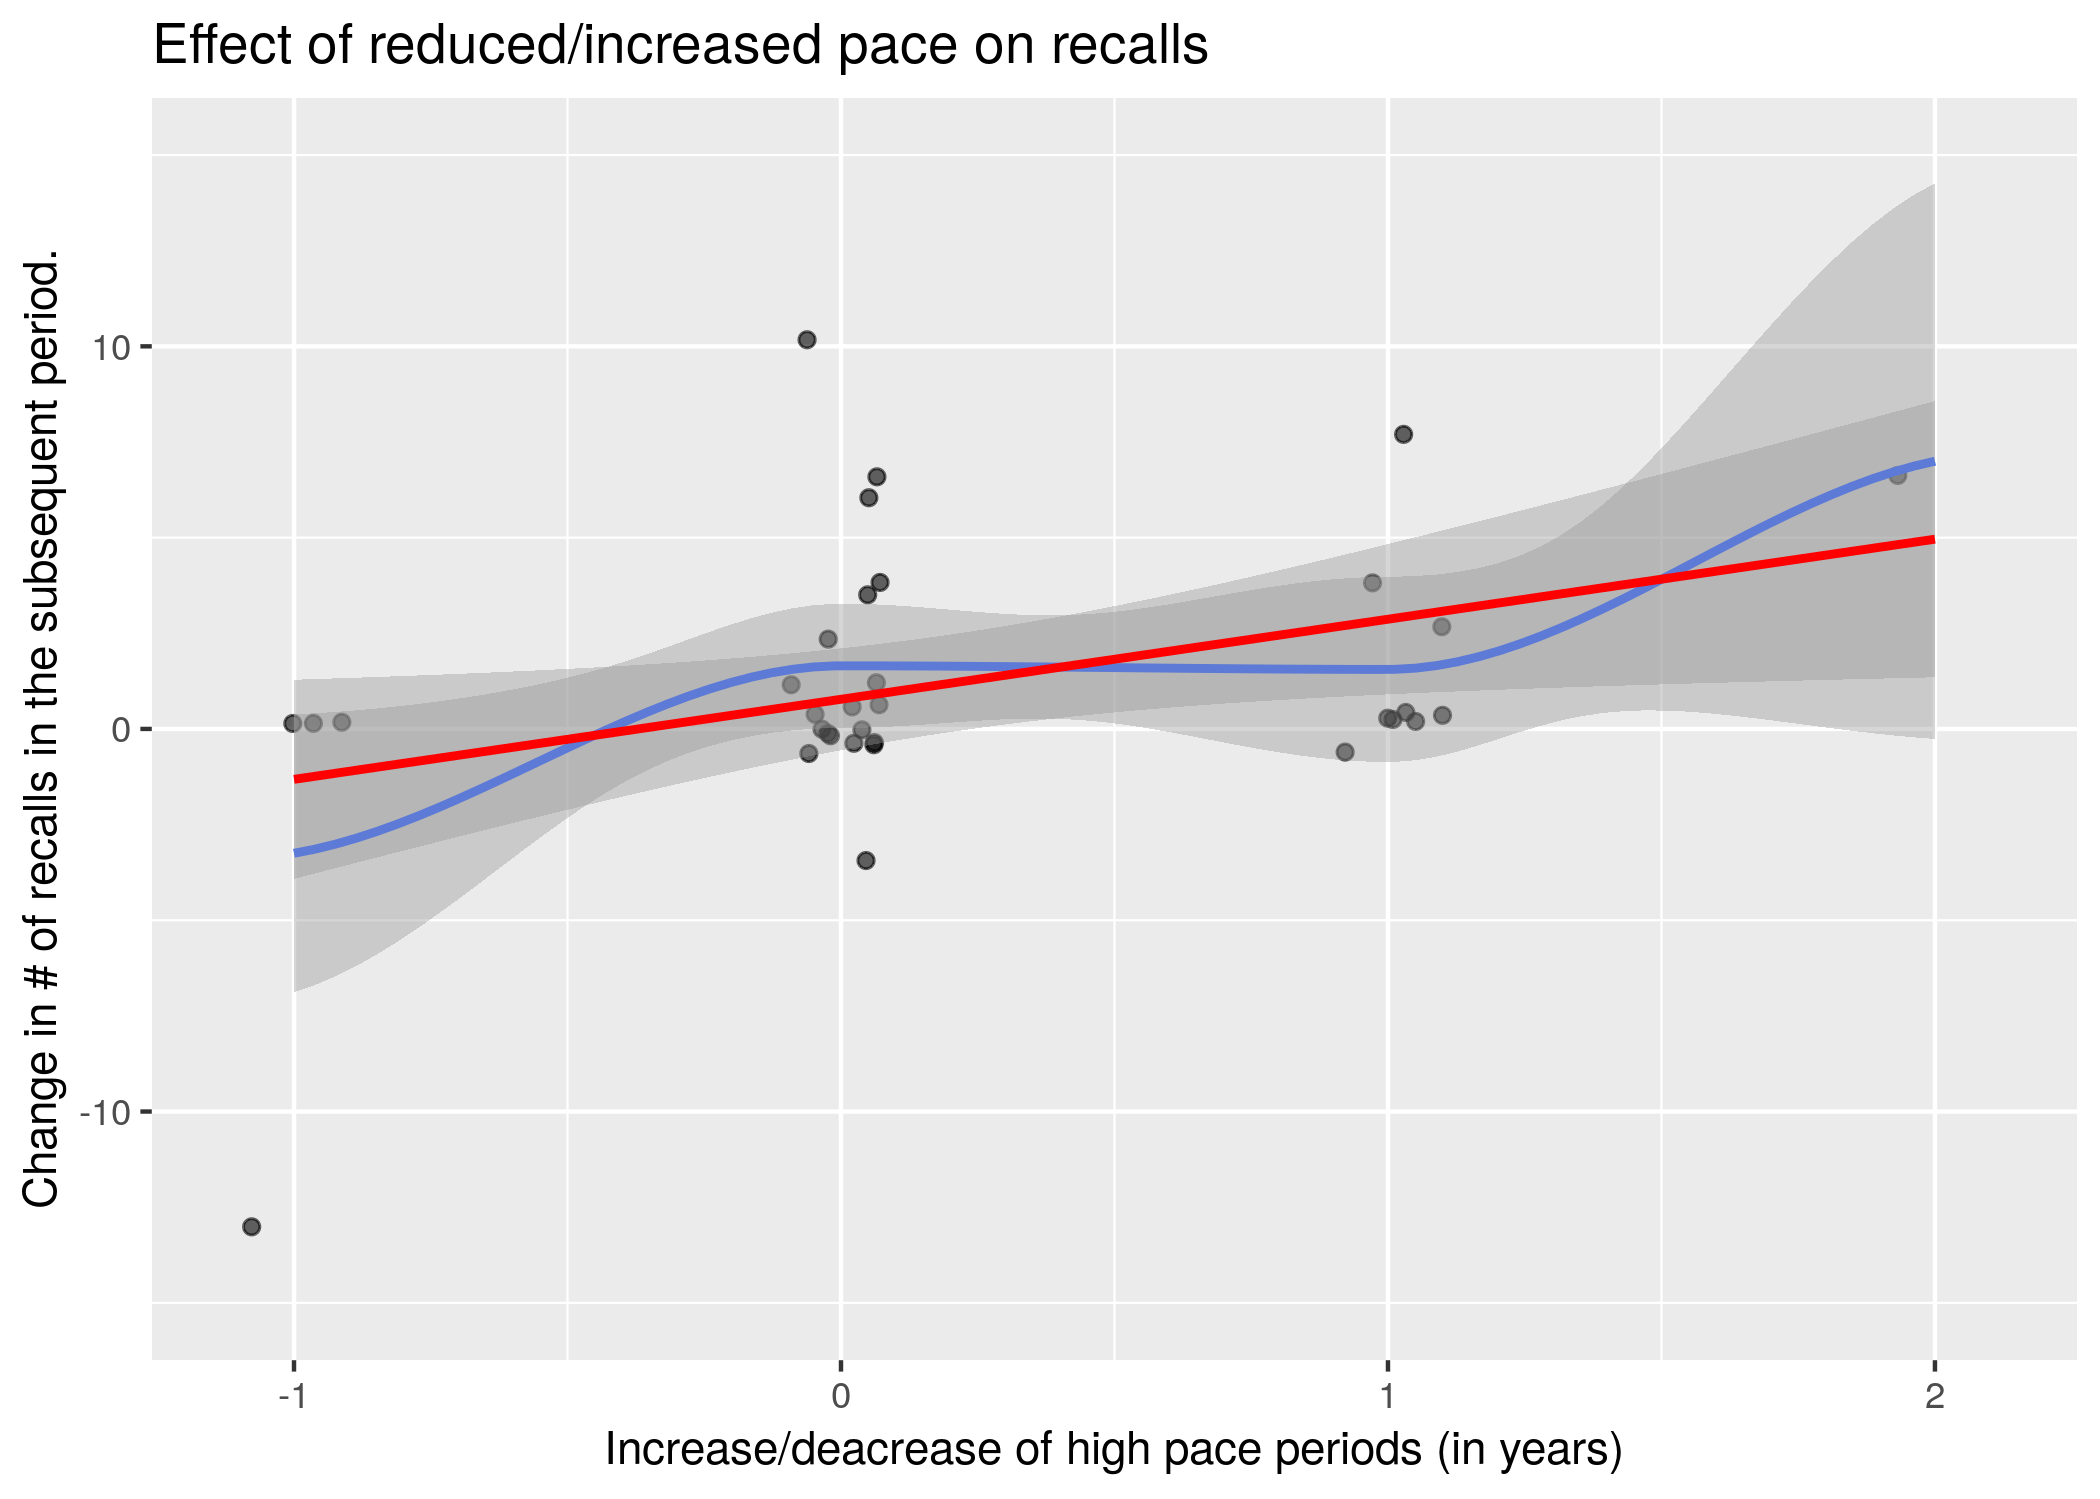
\includegraphics{illustrations/graph1.png}
\end{figure}

\begin{figure}
	\caption{}
	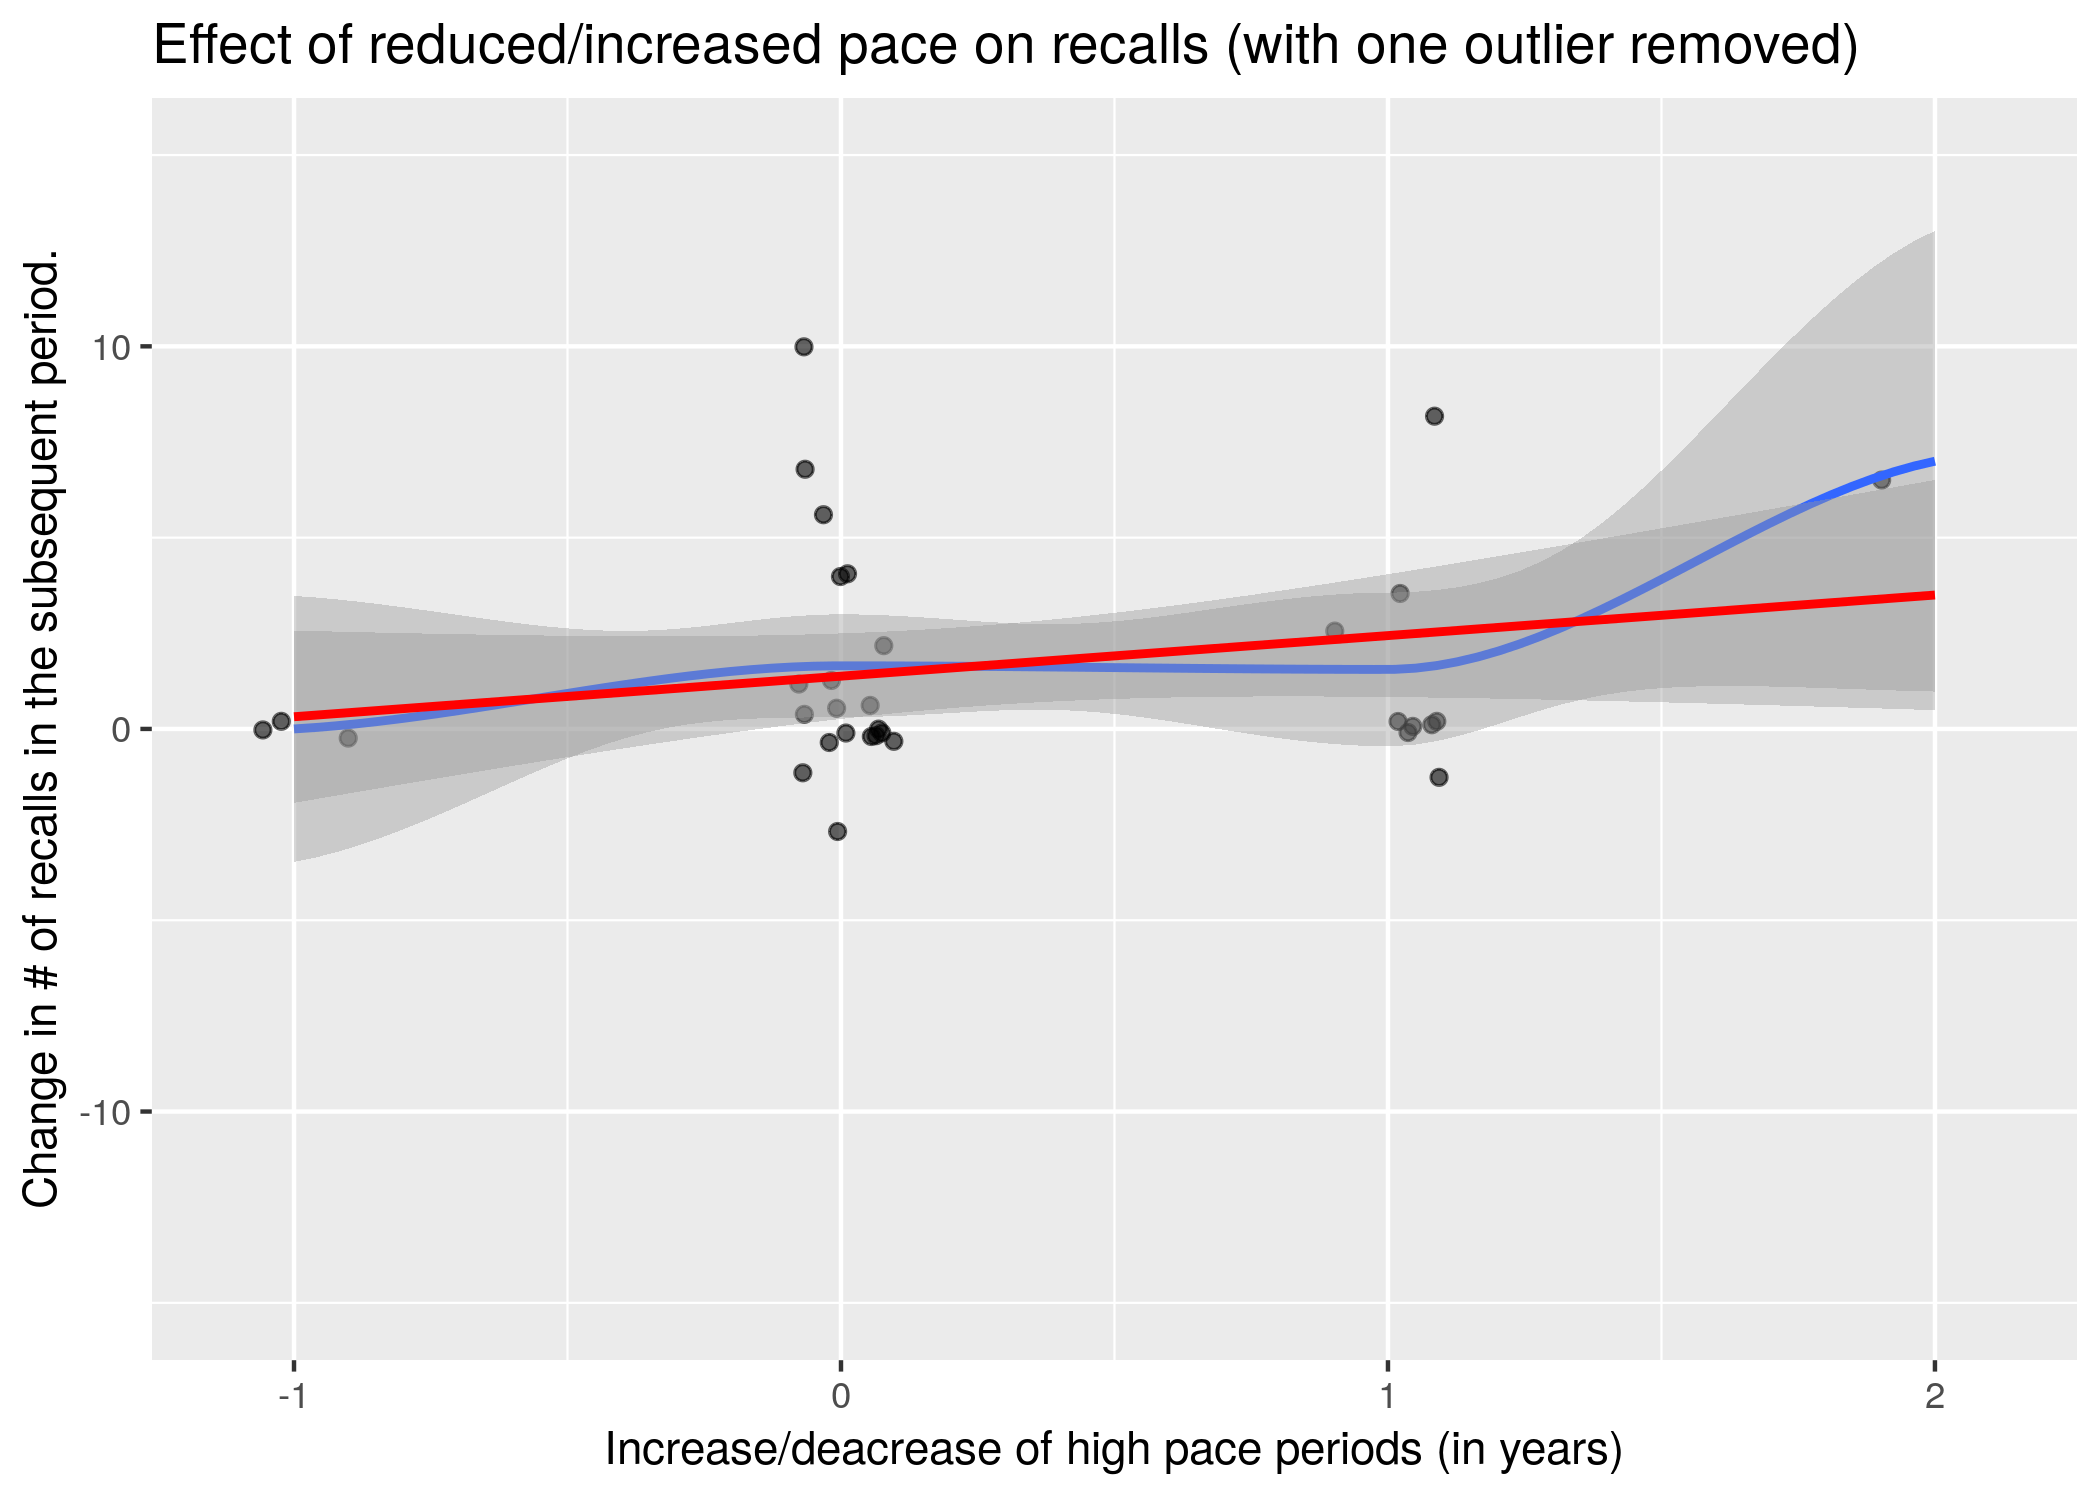
\includegraphics{illustrations/graph2.png}
\end{figure}

\begin{figure}
	\caption{}
	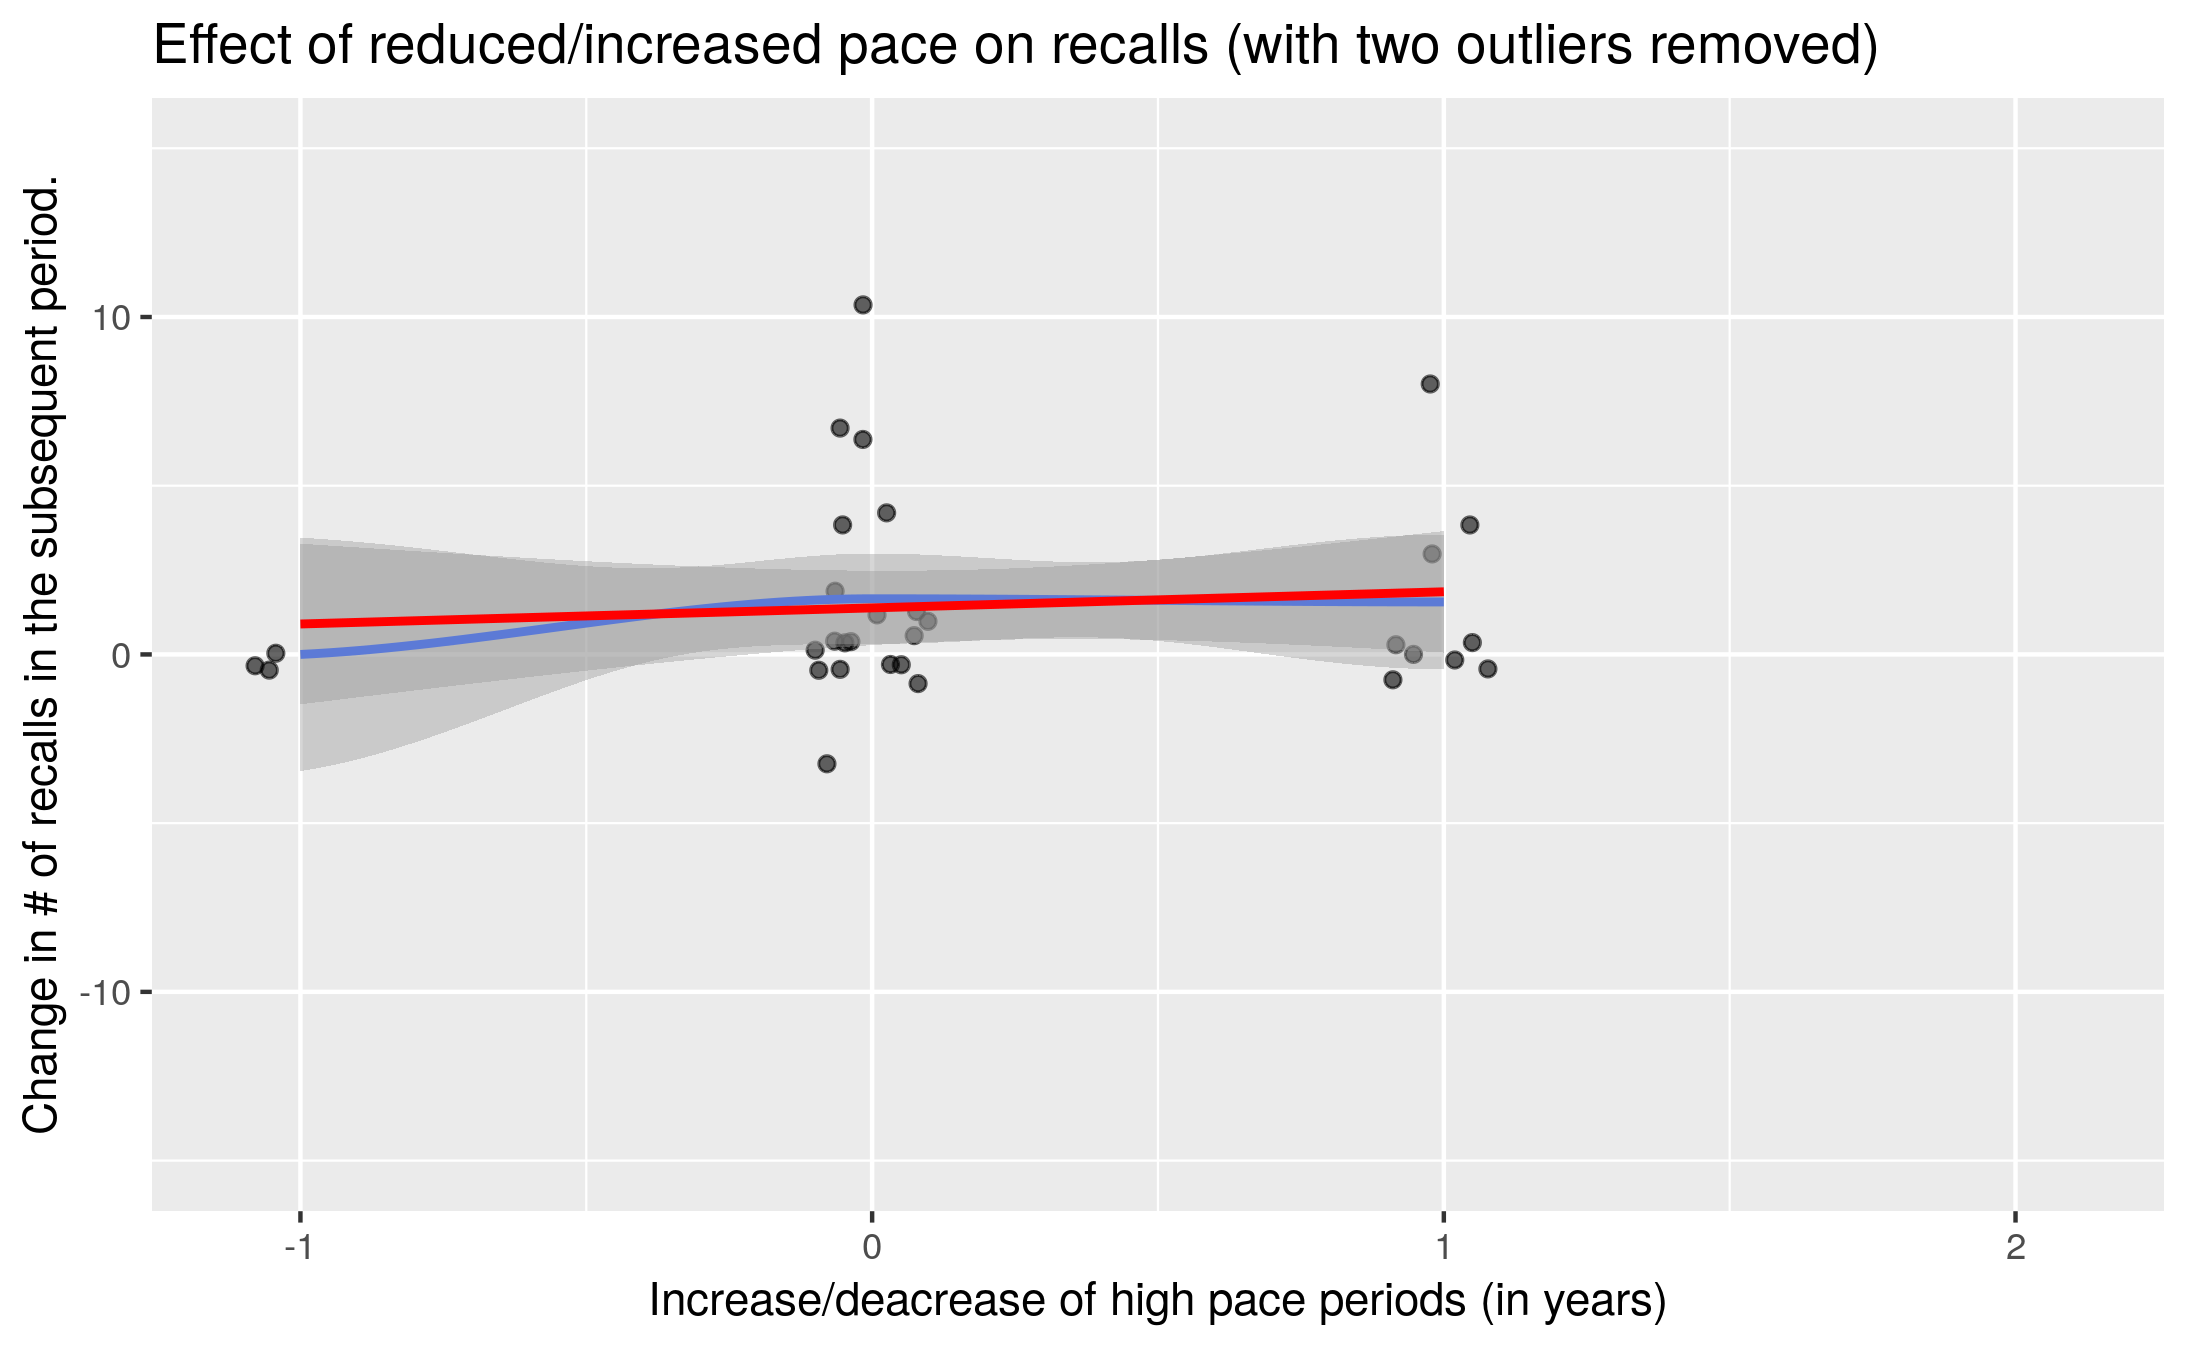
\includegraphics{illustrations/graph3.png}
\end{figure}



\section{Conclusion}

We have initially obtained some interesting results, but the inclusion of a year dummy made this effect disappear. Further, the results seem to be largely driven by two outliers. Moving forward, we want to test the our results on a larger dataset to gain more certainty. Some other limitations of the dataset can be rectified. More historical data on recalls is available. Further, better merging of the dataset might make some more of the data we have already collected available for analysis. Further, we have so far removed missing cases, instead, we could manually collect the missing data. Finally, more control variables might be available and allow us to better isolate the effect of pace, for instance R\&D or a variable that similarly captures exploration. In addition, there are some alternative data sources for our independent variable, top management turnover, such as BoardEx and Capital IQ.
\bibliography{bibliography}
	
\end{document}